\begin{homeworkProblem}[17][Blood $CO_2$ and Ventilation]
\begin{enumerate}
% Solution 17(a)
\item The old model supposes that the loss of $CO_2$ in only related to
ventilation. However, $CO_2$ can also diffuse spontaneously from high
concentration region to low concentration region. The new model includes this
factor.

% Solution 17(b)
\item The system of equations for $C_n$ and $V_n$ is \begin{align}
    C_{n+1} &= C_{n} - \beta V_nC_n + m\\
    V_{n+1} &= \alpha C_n.
\end{align}
Writing it as a single equation that only depends on $C_n$: \begin{equation}
    C_{n+1} = C_{n} - \alpha\beta C_n C_{n-1} + m \label{eq:CO2_next}
\end{equation}

% Solution 17(c)
\item Suppose $\bar C = C_{n+1} = C_n = C_{n-1}$, substituting $\bar C$ into
\eqref{eq:CO2_next} gives: \[
    \begin{aligned}
    \bar C &= \bar C - \alpha\beta\bar C^2 + m\\
    \bar C^2 &= m/\alpha\beta\\
    \bar C &= \sqrt{m/\alpha\beta} = \bar V/\alpha
    \end{aligned}
\]
To determine whether it's stable or not, we need to make the absolute value of
the roots of the characteristic function smaller than 1: \[
    \lambda^2 - b \lambda + c = 0
\]
where \[
    \begin{aligned}
        b &= \left.\pderiv{f}{C}\right|_{\bar C, \bar V} +
        \left.\pderiv{f}{V}\right|_{\bar C, \bar V} \\
        c &= \left.\pderiv{f}{C}\right|_{\bar C, \bar V}
        \left.\pderiv{g}{V}\right|_{\bar C, \bar V} -
        \left.\pderiv{f}{V}\right|_{\bar C, \bar V}
        \left.\pderiv{g}{C}\right|_{\bar C, \bar V}
    \end{aligned}
\]
Here \[
    \begin{aligned}
        f(C, V) &= C - \beta CV + m\\
        g(C, V) &= \alpha C
    \end{aligned}
\]
So \[
    \begin{aligned}
        b &= (1- \beta \bar V) = 1 - \sqrt{\alpha\beta m}\\
        c &= -\alpha(-\beta \bar C) = \sqrt{\alpha\beta m}
    \end{aligned}
\]
Recall that we derived in the book that if both eigenvalues have magnitude less
than 1, then \[
    \left\{
    \begin{aligned}
        &2 > 1 + c > |b|, & b^2 - 4c > 0\\
        &1 > c > |b/2|^2, & b^2 - 4c < 0
    \end{aligned}
    \right.
\]
Either way, when $c = \sqrt{\alpha\beta m} < 1$, both inequities hold. So
if we want the steady state to be stable, we need to have \[
    m\alpha \beta < 1
\]

% Solution 17(d)
\item We can have oscillation when the characteristic equation has complex
eigenvalues. To make this happen, we need to have \[
    b^2 - 4c = (1 - \sqrt{m\alpha\beta})^2 - 4\sqrt{m\alpha\beta} < 0
\]
Substitute $x = \sqrt{m\alpha\beta}$, then we should have \[
    x^2 - 6x + 1 < 0
\]
Solving this inequity gives \[
    3 - 2\sqrt{2} < x < 3+2\sqrt{2}
\]i.e., when we have$|x-3| < 2\sqrt{2}$, where $x = \sqrt{m\alpha\beta}$, there
will be oscillation in $V_n$ and $C_n$.

% Solution 17(e)
\item The system of equations will look like \begin{align}
    C_{n+1} &= C_n - \beta V_nC_n + m \label{eq:new_CO2_next}\\
    V_{n+1} &= \frac{V_{\max}C^\mathcal{l}_n}{K^{\mathcal{l}}+C^\mathcal{l}_{n}}
    \label{eq:new_ventilation_next}
\end{align}
It's trivial to show that if we write \eqref{eq:new_ventilation_next} as 
\begin{equation}
    V_{n} = \frac{
        V_{\max}C^\mathcal{l}_{n-1}}{K^{\mathcal{l}}+C^\mathcal{l}_{n-1}}
    \label{eq:new_ventilation}
\end{equation}
and plug \eqref{eq:new_ventilation} to \eqref{eq:new_CO2_next}, then we'll have
\begin{equation}
    C_{n+1} = C_n - \beta \frac{
        V_{\max}C^\mathcal{l}_{n-1}C_n}{K^{\mathcal{l}}+C^\mathcal{l}_{n-1}}
        + m
\end{equation}

% Solution 17(f)
\item The relationship between $\mathcal{S}(C)$ and $\mathcal{l}$ is shown in
Figure \ref{fig:CO2_sensitivity}. $K$ is chosen to be $50$.
\begin{SCfigure}[8][h]
    \centering
    \caption[The relationship between $\mathcal{S}(C)$ and $\mathcal{l}$]{
        The relationship between $\mathcal{S}(C)$ and $\mathcal{l}$.
    }
    \label{fig:CO2_sensitivity}
    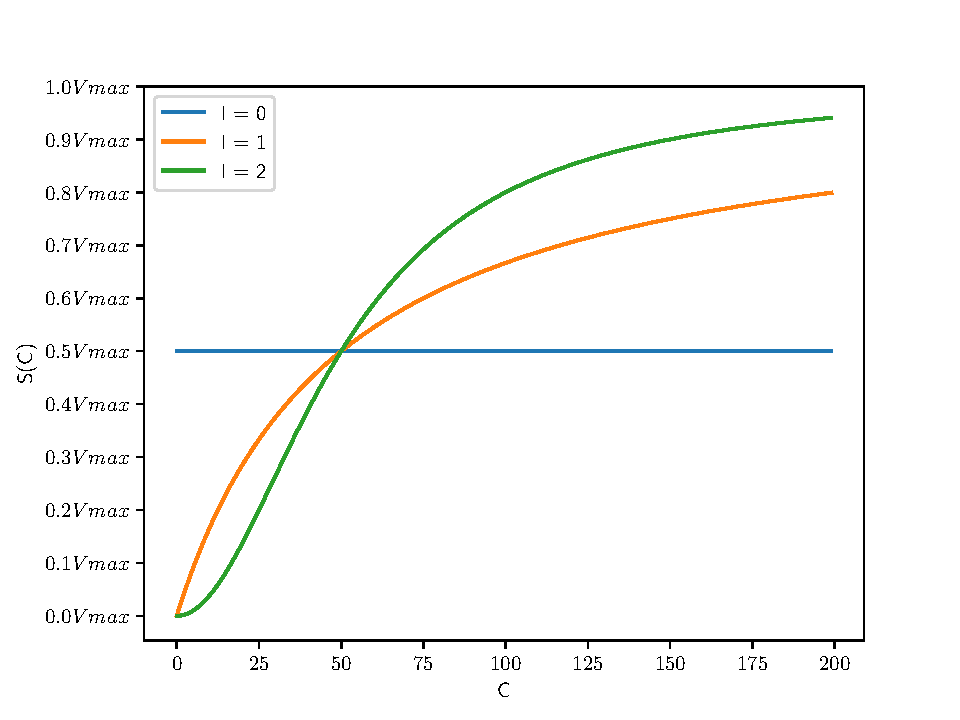
\includegraphics[scale=0.6]{fig/fig17(f).pdf}
\end{SCfigure}

% Solution 17(g)
\item \unsolved

% Solution 17(h)
\item \unsolved\\ When $\mathcal{l} = 1$, \[\begin{aligned}
    C_{n+1} &= C_n - \beta V_nC_n + m\\
    V_{n+1} &= \frac{V_{\max}C_n}{K+C_{n}}
\end{aligned}\]
and \begin{equation}
    C_{n+1} = C_n - \beta \frac{V_{\max}C_{n-1}C_n}{K+C_{n-1}}+ m
    \label{eq:stable}
\end{equation}
Suppose $\bar C = C_{n+1} = C_n = C_{n-1}$ and plug it into \eqref{eq:stable},
\[
    \begin{aligned}
        &\bar C - \beta \frac{V_{\max}\bar C^2}{K + \bar C} + m = \bar C\\
        &\frac{\bar C^2}{K + \bar C} = \frac{m}{\beta V_{\max}}\\
        &\bar C^2-\frac{m}{\beta V_{\max}}\bar C - \frac{m}{\beta V_{\max}}K = 0
    \end{aligned}
\]
Let $\delta = \frac{m}{\beta V_{\max}}$, then \[
    \begin{aligned}
        \bar C &= \frac{1}{2}\left(\delta \pm \sqrt{\delta + 4K \delta}\right)\\
        \bar V &= \frac{V_{\max} \bar C}{K + \bar C} 
    \end{aligned}
\]
We need to make the roots for the characteristic equation have a magnitude $< 1$
again:
\[
    \lambda^2 - b\lambda + c = 0
\]
where \[
    \begin{aligned}
        b &= \left.\pderiv{f}{C}\right|_{\bar C, \bar V} +
        \left.\pderiv{f}{V}\right|_{\bar C, \bar V} \\
        c &= \left.\pderiv{f}{C}\right|_{\bar C, \bar V}
        \left.\pderiv{g}{V}\right|_{\bar C, \bar V} -
        \left.\pderiv{f}{V}\right|_{\bar C, \bar V}
        \left.\pderiv{g}{C}\right|_{\bar C, \bar V}
    \end{aligned}
\]
Here \[
    \begin{aligned}
        f(C, V) &= C - \beta CV + m\\
        g(C, V) &= \frac{V_{\max}C}{K+C}
    \end{aligned}
\]
So \[
    \begin{aligned}
        b &= (1- \beta \bar V) = 1- \frac{\beta V_{\max}\bar C}{K+\bar C}\\
        c &= \frac{\beta  V_{\max} K \bar C}{(K + \bar C)^2}
    \end{aligned}
\]
Recall again that we derived in the book that if both eigenvalues have magnitude
less than 1, then \[
    \left\{
    \begin{aligned}
        &2 > 1 + c > |b|, & b^2 - 4c > 0\\
        &1 > c > |b/2|^2, & b^2 - 4c < 0
    \end{aligned}
    \right.
\]


% Solution 17(i)
\item \unsolved

\end{enumerate}
\end{homeworkProblem}